\section{Einfluss der grundlegenden Indizes}\label{auswertung:basic_indizes}
%TODO
% Row with or without indices
% Column with or without indices
\iffalse
\begin{figure}[H]
    \centering
    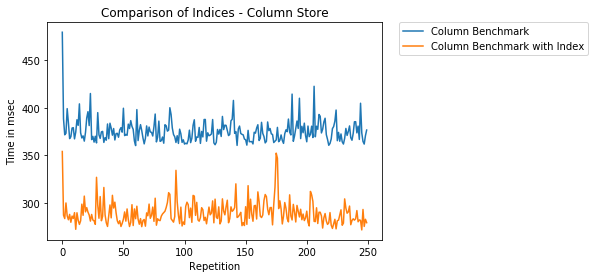
\includegraphics[width=0.49\textwidth]{col_ind.png}
    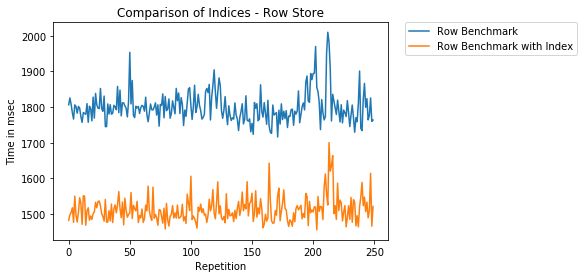
\includegraphics[width=0.49\textwidth]{row_ind.png}
    \caption{Gesamtergebnis für Row- und Columnstore.}
	\label{fig:ind_overall}
\end{figure}
\fi

Im folgenden soll die Auswirkung grundlegender Indizes auf die Laufzeit der Queries untersucht werden. Die angelegten Indizes finden sich in 
\autoref{fig:ind_layout} zeigt das DB-Layout mit Indizes. Die \textbf{fett} markierten Attribute sind Felder, auf die Indizes angelegt wurde.



\begin{figure}[H]
    \centering
    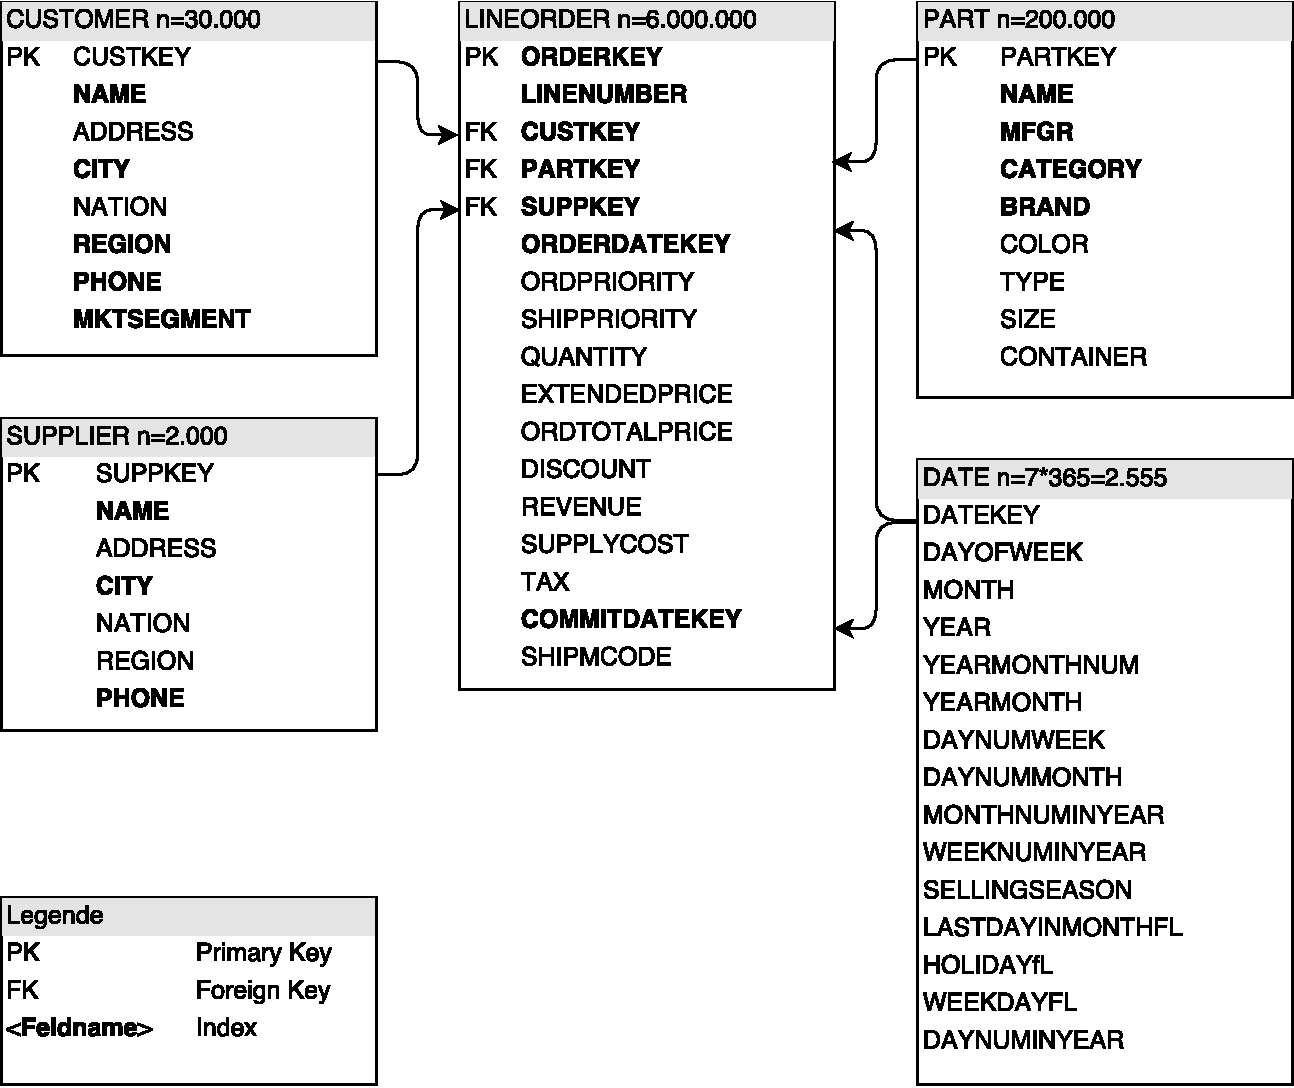
\includegraphics[width=0.49\textwidth]{images/ssbm_basic}
    \caption{Übersicht des DB-Layouts mit Indizes.}
	\label{fig:ind_layout}
\end{figure}

Um die Indizes anzulegen wurde der folgende Code ausgeführt:
\begin{Verbatim}
CREATE INDEX idx_c_name ON customer(C_Name);
CREATE INDEX idx_c_city ON customer(C_City);
CREATE INDEX idx_c_region ON customer(C_Region);
CREATE INDEX idx_c_phone ON customer(C_Phone);
CREATE INDEX idx_c_mktsegment ON customer(C_MktSegment);

CREATE INDEX idx_p_name ON part(P_Name);
CREATE INDEX idx_p_mfgr ON part(P_MFGR);
CREATE INDEX idx_p_category ON part(P_Category);
CREATE INDEX idx_p_brand ON part(P_Brand);

CREATE INDEX idx_s_city ON supplier(S_City);
CREATE INDEX idx_s_name ON supplier(S_Name);
CREATE INDEX idx_s_phone ON supplier(S_Phone);

CREATE INDEX idx_lo_orderkey_lo_linenumber ON lineorder(LO_OrderKey, LO_LineNumber);
CREATE INDEX idx_lo_custkey ON lineorder(LO_CustKey);
CREATE INDEX idx_lo_suppkey ON lineorder(LO_SuppKey);
CREATE INDEX idx_lo_partkey ON lineorder(LO_PartKey);
CREATE INDEX idx_lo_orderdatekey ON lineorder(LO_OrderDateKey);
CREATE INDEX idx_lo_commitdatekey ON lineorder(LO_CommitDateKey);
\end{Verbatim}

\subsection{Grundlegende Untersuchung für Columnstore}
\begin{table}[H]
\centering
    \begin{tabularx}{\textwidth}{lrrr}
        \toprule
        Merkmal             &   Col[ms]    &    Col Index[ms] & Abweichung[\%]\\
        \toprule
        Samples             &   250        &   250      &       \\
        \midrule    
        Median              &   373        &   286      & 23.3\%\\
        Average             &   376        &   289      & 23.1\%\\
        \bottomrule
    \end{tabularx}
\caption{Vergleich der Ergebnisse mit und ohne grundlegende Indizes für Columnstore.}
\label{tab:basic_index_col}
\end{table}

Durch hinzufügen der grundlegenden Indizes wurde der Benchmark
für Columstores sowohl im Schnitt als auch im Median schneller.
Im Schnitt wurde er 23,1\%, im Median um 23,3\% schneller.

Diese Ergebnisse sind interessant, da in der Regel davon ausgegangen wird, 
dass bei Columnstores kein großartiges Optimierungspotenzial durch Indizes vorhanden ist.
Um herauszufinden, warum trotzdem eine deutliche Verbesserung messbar ist,
wird der Query-Execution Plan des Subqueries mit der deutlichsten Verbesserung
im folgenden untersucht.

Schaut man sich die Ergebnisse für jede Query Gruppe (siehe \autoref{tab:qg_c}) an, so sind 
deutliche Verbesserungungen sind bei den Queries der Gruppen 1 und 3 festzustellen. 
Hier hat sich die Laufzeit um 35\% bzw. sogar 41\% reduziert. 
Die Queries dieser Gruppe werden im Detail untersucht, um geeignete Kandidaten 
für die Analyse des Execution-Plans zu finden.

\begin{table}[H]
    \centering
    \begin{tabularx}{\linewidth}{crrr}
        \toprule
        Benchmarkgruppe & Col[ms]   & Col Index[ms] & Laufzeitreduzierung[ms|\%]\\
        \toprule
        Q1              & 104.7       & 68.5            & 36.2 | 34.5\%\\
        Q2              & 62.1        & 59.7            & 2.4 |  03.8\%\\
        Q3              & 96.2        & 54.8            & 41.4 | 40.8\%\\
        Q4              & 112.4       & 106.3           & 6.1 |  05.4\%\\
        \bottomrule
    \end{tabularx}
	\caption{Durchschnittslaufzeit für jede Benchmarkgruppe für Columnstore.}
    \label{tab:qg_c}
\end{table}

Hier sind besonders bei Query 1.2 und 3.4 interessant, da diese die größte 
Verbesserung in ihrer Gruppe vorweisen können, siehe \autoref{tab:q1_q3_col}. 
Die Laufzeit wurde um 64\% für Query 1.2 und um mehr als 90\% für Query 3.4 
reduziert. Woher diese Verbesserung kommen, soll im Folgenden durch die Analyse 
der Execution-Pläne von Query 1.2 und 3.4 geklärt werden.

\begin{table}[H]
    \centering
    \begin{tabularx}{\linewidth}{crrr}
        \toprule
        Benchmark           & Col[ms]       & Col Index[ms] & Laufzeitreduzierung[ms|\%]   \\
        \toprule
        Q1.1                & 36.1          & 36.4          & -0.3 | -0.8\%                \\
        Q1.2                & 47.8          & 16.8          & 31.0 | 64.8\%                 \\
        Q1.3                & 21.3          & 14.1          & 7.2 | 33.8\%                \\
        \midrule
        Q3.1                & 31.3          & 31.6          & -0.3 | -0.9\%                \\
        Q3.2                & 24.0          & 18.9          & 5.1 | 21.2\%                 \\
        Q3.3                & 21.3          & 2.1           & 19.2 | 90.1\%                \\
        Q3.4                & 20.5          & 1.6           & 18.9 | 92.1\%                \\
        \bottomrule
    \end{tabularx}
\caption{Durchschnittslaufzeit für Benchmarkgruppen 1 und 3 für Columnstore.}
\label{tab:q1_q3_col}
\end{table}

\subsubsection{Analyse von Query 1.2}
\textbf{Hinweis:} Die Ergebnisse in diesem Abschnitt basieren auf Ausführung auf einem PC mit einer Intel Xeon 1230 V3 CPU mit 16GB DDR3 RAM. Die VM hatte 4 Kerne und 8GB RAM zur Verfügung.
%https://archive.sap.com/discussions/thread/3429357

\setlength\intextsep{0pt}
\begin{wraptable}{r}{0.5\textwidth}
    \centering
    \begin{tabular}{cc}
        Col [ms]       & Col Index [ms]    \\
        \toprule
         16          & 6         \\   
    \end{tabular}
	\caption{Durchschnittslaufzeit für Query 1.2 bei Columnstore.}
    \label{tab:olap_q12}
\end{wraptable}

Bei Query 1.2 gibt es einen deutlichen Unterschied zwischen Index und kein Index. Hierbei kann der Index auf LO\_OrderDateKey für den JOIN genutzt werden und beschleunigt diesen somit.
Außerdem wird die Berechnung \textbf{sum(lo\_extendedprice*lo\_discount)} deutlich beschleunigt. Warum ist allerdings nicht klar, denn auf diese Felder wurde kein Index angelegt.


Schaut man sich genauer an, was an dieser Stelle passiert, so werden die gleichen Operationen auf die gleichen Datenmengen angewandt, allerdings sind die Operationen \textbf{mit} Index deutlich schneller.\footnote{Die letzte Zahl scheint jeweils die Laufzeit in ms zu sein, aber eine genaue Erklärung dieser Werte war leider nicht zu finden.}
\begin{lstlisting}[breaklines, caption=Ohne Index]
<executePop(
  <lockInputs(num=3,)=0.00>
    <calculateOnAttr(
      <calculateWithAggregation(rows=4301,inputs=2,outputs=1,)=8.04>
    rows=4301,outputs=1,)
  =8.15>
)=11.61>
\end{lstlisting}

\begin{lstlisting}[breaklines, caption=Mit Index]
<executePop(
  <lockInputs(num=3,)=0.00>
    <calculateOnAttr(
      <calculateWithAggregation(rows=4301,inputs=2,outputs=1,)=1.03>
    rows=4301,outputs=1,)
  =1.10>
)=1.18>
\end{lstlisting}

\subsubsection{Analyse von Query 3.4}
\textbf{Hinweis:} Die Ergebnisse in diesem Abschnitt basieren auf Ausführung auf einem PC mit einer Intel Xeon 1230 V3 CPU mit 16GB DDR3 RAM. Die VM hatte 4 Kerne und 8GB RAM zur Verfügung.

Bei der Analyse des Query-Execution Plans zeigt sich schnell,
woher die große Geschwindigkeitssteigerung kommt.
Query 3.4 bildet einen Join von Lineorder auf Customer,
Supplier und Dim\_Date. 
Dieser Join erfolgt jeweils über den Fremdschlüssel in Lineorder.
Ohne Indizes ist dieser Join ausschlaggebend für die Laufzeit des Querys.
Durch anlegen von Indizes auf alle Fremdschlüssel,
kann der Join deutlich schneller ausgeführt werden.
Den größten Vorteil hat hier der Index auf LO\_Suppkey.

Der Execution Plan ohne Indizes ist in \autoref{execution-plan:before-index}, sowie \autoref{exec:q3.4-col-no}
zu finden und der Execution Plan mit Indizes ist in \autoref{execution-plan:after-index},sowie \autoref{exec:q34-col-index} zu finden.

Query 3.1 im Vergleich nutzt zwar auch Fremdschlüssel, um einen Join zu bilden,
allerdings sind hier die nicht indizierten Felder \verb+S_Region+, \verb+D_Year+,
\verb+C_Nation+ und \verb+S_Nation+ in der Where- und der Group by-Klausel gelistet,
wodurch eine Geschwindigkeitsverbesserung nicht möglich ist.

Auch bei Columnstores scheinen sinnvoll angelegte Indizes also einen deutlichen Unterschied zu machen.

\subsubsection{Fazit für Columnstores}
Auch Columnstores können durch geschickt gewählte Indizes deutlich beschleunigt werden. Erwartet man nur wenige schreibende Zugriffe auf eine Tabelle kann es also durchaus Sinn machen, sinnvolle Indizes anzulegen.
%https://archive.sap.com/discussions/thread/3277920

\subsection{Grundlegende Untersuchung für Rowstore}
Durch hinzufügen der grundlegenden Indizes wurde der Benchmark
für Rowstores sowohl im Schnitt als auch im Median schneller.
Im Schnitt wurde er 15,9\%, im Median um 15,9\% schneller.

Die Verbesserungen beim Rowstore fallen, zumindest relativ gesehen, deutlich geringer als beim Columnstore (23,1\% und 23,3\%) aus.

\begin{table}[H]
    \begin{tabularx}{\textwidth}{lrrr}
        \toprule
        Wert                & Row[ms] & Row Index[ms]   & Abweichung [\%]\\
        \toprule
        Samples             & 250      & 250            &   ---    \\
        \midrule
        Median              & 1794     & 1508           &  15.9\%     \\
        Average             & 1800     & 1513           &  15.9\%     \\
        \bottomrule
    \end{tabularx}
\caption{Vergleich der Ergebnisse mit und ohne grundlegende Indizes für Rowstore.}
\label{tab:basic_index_row}
\end{table}

Schaut man sich die Veränderung der Laufzeit für die einzelnen Querygruppen, so fällt auf, dass Gruppe 1 und 2 deutlich von den Indizes profitieren, Gruppe 3 so gut wie gar nicht und Gruppe 4 wurde sogar \textbf{deutlich} langsamer.
Um zu analysieren, woran diese deutlichen Verbesserungen/Verschlechterungen liegen, wird aus Gruppe 2 und 4 jeweils der Query mit der größten Änderung analysiert.

\begin{table}[H]
    \begin{tabularx}{\linewidth}{lrrrr}
        \toprule
                            &   q1          &   q2      &	q3      & q4          \\
        \toprule
        Row[ms]	            &	423	        &	352	    &	519	    & 507	      \\
        Row Index[ms]       &   170         &   90	    &   473	    & 780	      \\
        Verbesserung[ms]    &   253         &   120     &   46      & -273        \\
        Verbesserung[\%]    &   59,8\%      &   74,4\%  &   8,8\%   & -53,8\%     \\    
\bottomrule
\end{tabularx}
\caption{Durchschnittslaufzeit jeder Querygruppe. n=250}
\label{tab:basic_index_row_q}
\end{table}



\subsection{Analyse der Queries aus Gruppe 2}

Wie in \autoref{tab:q2_row} zu sehen, profitieren alle 3 Queries recht deutlich von den Indizes. 
Die deutlichste Änderung gibt es jedoch bei Query 2.3, welcher im folgenden im Detail untersucht werden soll.

\setlength\intextsep{0pt}
\begin{table}[H]
    \begin{tabularx}{\linewidth}{lrrr}
        \toprule
                        & q2.1  &	q2.2    &	q2.3 \\
        \toprule
        Row[ms]	        & 139	&	111	    &	102  \\
        Row Index[ms]   & 73	&   16	    &   4    \\
        Verbesserung[ms]  & 66    &   95      &   98   \\
        Verbesserung[\%]  & 47.4\%  &   85.5\%    &   96.0\% \\    
\bottomrule
\end{tabularx}
\caption{Laufzeiten der Queries aus Gruppe 2.}
\label{tab:q2_row}
\end{table}

Der Query Execution Plan für Query 2.3 ohne Index wird in \autoref{fig:q23_r}, der Plan für Query 2.3 mit Index in \autoref{fig:q23_r_I}, dargestellt.

Die Ursache für die große Verbesserung bei Query 2.3 lässt sich sehr leicht erkennen:

Anstatt die Tabellen Lineorder und Part erst über einen Table Scan zu durchsuchen und anschließend über einen Hash-Join zu verknüpfen,kann nun der einerseits der Index
auf PartKey in Lineorder und Part für den Join genutzt werden. Außerdem kann der Index auf P\_Brand genutzt werden, um Part schneller zu filtern. 

Die Laufzeit für diesen einzelnen Schritt kann von 169,7ms auf 2ms reduziert werden.


\subsection{Analyse der Queries aus Gruppe 4}

Wie in \autoref{tab:q4_row} zu sehen, wird Query 4.3 sogar schneller durch die Indizes. 
Die beiden anderen Queries werden jedoch deutlich langsamer. Die deutlichste Änderung 
gibt es bei Query 4.1, welcher im folgenden im Detail untersucht werden soll.

\setlength\intextsep{0pt}
\begin{table}[H]
    \begin{tabularx}{\linewidth}{lrrr}
        \toprule
                        & q4.1      &	q4.2        &	q4.3       \\
        \toprule
        Row[ms]	        & 200	    &	175	        &	125        \\
        Row Index[ms]   & 421	    &   320	        &   78          \\
        Verbesserung[ms]  & -221      &   -145        &   47         \\
        Verbesserung[\%]  & -110\%    &   -82,8\%     &   37,6\%       \\    
\bottomrule
\end{tabularx}
\caption{Laufzeiten der Queries aus Gruppe 4.}
\label{tab:q4_row}
\end{table}

Der Query Execution Plan für Query 4.1 ohne Index wird in \autoref{fig:q41_r}, der Plan für Query 4.1 mit Index in \autoref{fig:q41_r_I}, dargestellt.

Auf den ersten Blick scheinen die Indizes Wirkung zu zeigen: Anstatt Table Scans in Kombination mit Hash-Joins zu Nutzen werden Index Search und Index Join verwendet.

Allerdings wird die Bedingung auf Custkey immer noch über einen Hash Join erfüllt. Bei der Version ohne Index sind die Treffermengen ~400 und ~1.2 Millionen.
Mit Index sind die Treffermengen ~6000 und ~1.1 Millionen.

%https://de.wikipedia.org/wiki/Joinalgorithmen
Für die durchschnittliche Laufzeit des  Hash Joins gilt:\cite{hash}
\begin{equation}
    \mathcal{O}(m+n)
\end{equation}

Die Laufzeiten sollten also in etwa gleich sein, wenn der Join ohne Index nicht sogar langsamer sein sollte.

Trotzdem benötigt der Join ohne Index nur 168ms, mit Index werden 283ms benötigt.
Warum die Laufzeiten dennoch so stark voneinandern abweichen, ist nicht klar. Möglicherweise ist 
die Hashtabelle auf die Treffermenge 6000 Einträgen zu groß, um komplett im Hauptspeicher zu liegen.
Überprüft wurde dies jedoch nicht.

Der Unterschied ist beim Hash-Join zwar am auffälligsten, allerdings sind auch viele andere Schritte, wie zum Beispiel die Suche auf Lineorder, bei der Version ohne Index schneller, was sich in Summe in dem großen Laufzeitunterschied niederschlägt.


\subsection{Fazit für Rowstore}
Auch Rowstores können durch geschickt gewählte Indizes deutlich beschleunigt werden. Sie profitieren zwar nicht ganz so stark wie Columstores, werden aber doch merklich schneller.  
Allerdings scheint es auch Fälle zu geben, in denen Indizes deutliche Verschlimmbesserungen darstellen. Von blind angelegten Indizes ist also abzuraten.

\section{Fazit}
Sowohl Columnstores als auch Rowstores könen durch Indizes nochmals teils deutlich 
beschleunigt werden. Bei Rowstores gab es jedoch auch Fälle, wo die Indizes den Query deutlich verlangsamten.
Doch auch mit Indizes liegen Rowstores immer noch weit hinter Columnstores. 